\chapter{Results}
\label{Chapter4}
\section{Baseline models}
The simplest model for the gust factor is to guess the average gust factor for all available observations, i.e. use no variables from the training data. A slightly better model is obtained by using the wind speed as a training feature, either through regression or NN training. The MAPEs for the constructed base models are shown in Table \ref{table:baseline_models}. The ws$_{15}$ model was obtained with NN training but regression produces an almost identical result.

\begin{table}[h]
  \caption[MAPE for baseline models]{MAPE for several lower limits on the reanalysis 15 m wind speed ($ws_{15}$). Note that the ws$_{15}$ model was only evaluated for the 10 m/s lower bound.}
    \label{table:baseline_models}
    \centering
    \begin{tabular}{lcc}
        \toprule
        Wind speed & \multicolumn{2}{c}{MAPE}\\ 
        limit $[m/s]$ & mean model & ws$_{15}$ model\\
        \midrule
        $\geq 0$ & 39.2\%  & \\
        $\geq 5$ & 28.1\%  & \\
        $\geq 10$ & 23.9\% & 17.2\%\\
        $\geq 15$ & 23.2\% & \\
        $\geq 20$ & 24.7\% & \\
        $\geq 25$ & 27.7\% & \\
        \bottomrule
    \end{tabular}
\end{table}

As the average wind speed increases, then the variability in gust as a percentage decreases\cite{mean_gust_HA_HO}. Therefore lower MAPE would be expected if the training data is restricted to higher wind speeds. This fact explains why several models were created for different lower bounds.

\section{Modeling for CARRA wind speed above 10 m/s}
As noted in Chapter \ref{Chapter1}, it is more important to predict accurate gust factor when it is windy than when the weather is calm. Therefore, at first, the data is restricted to ws$_{15} \geq 10$ m/s. The first constructed model incorporates the features temperature, pressure and wind direction at 15 m height. This gives a moderately reduced MAPE of 16.7\% compared with 17.2\% for the baseline ws$_{15}$ model. When the next pair of features, station altitude and transformed wind direction, is included, the MAPE is reduced considerably, down to 13.8\%. The atmospheric stability indicators, Ri and $N^2$, add little to the model performance, contrary to what might have been expected. When the atmosphere is unstable, wind gusts from higher up might be expected. However, another considerable performance increase is observed when digital elevation model (DEM) information is included, down to a MAPE of 12.0\%. This represents over 30\% reduction in the MAPE from the ws$_{15}$ baseline model.

\begin{table}[h]
    \caption[Model results for different sets of parameters.]{Showing the results of different models. Models defined by different sets of parameters, with increasing complexity. This table shows the feature importance as the loss decreases as more variables are added. Adding all height levels decreases the loss but very little.}
    \label{table:setsOfParams}
    \centering
    \begin{tabular}{lc}
        \toprule
        Model variables & MAPE\\
        \midrule
        Baseline constant & 23.9\%\\
        $ws_{15}$ & 17.2\%\\
        $[ws_{15}, t_{15}, p_{15}, wd_{15}]$ & 16.7\% \\
        $[ws_{15}, t_{15}, p_{15}, wd_{15}, \text{altitude}, twd]$ & 13.8\% \\
        $[ws_{15}, t_{15}, p_{15}, wd_{15}, \text{altitude}, twd, N^2, Ri]$ & 13.7\%\\
        $[ws_{15}, t_{15}, p_{15}, wd_{15}, \text{altitude}, twd, N^2, Ri]$ + DEM & 12.0\%\\
        $[ws_{15,250,500}, t_{15,250,500}, p_{15,250,500}, wd_{15,250,500}, \text{altitude}, twd, N^2, Ri]$ & 12.0\% \\
        \bottomrule
    \end{tabular}
\end{table}

The results show this. Several different wind speed intervals were used for the baseline model, as can be seen in table \ref{table:results}. This sets a goal. A model that does not significantly improve on this baseline suggests either failure to capture essential patterns in the data or that the data itself may lack the necessary information for substantial improvements upon the baseline. Using the previously described neural network architecture setups for each wind speed interval, with and without landscape elevation information, MAPE was determined. The results can be seen in Table \ref{table:results}.

\begin{table}[h]
    \caption[Model results for different wind speed limits]{MAPE for each average wind speed limit with and without landscape elevation in a 30° sector around the point of interest into the direction of the reanalysis wind. The influence of adding elevation data seems to reduce the error. The percentage error is higher for lower wind speeds and thus observing the error for different lower bound of wind speed will produce different results. This lower bound is determined using the reanalysis wind speed at 15 meters ($ws_{15}$).}
    \label{table:results}
    \centering
    \begin{tabular}{lccc}
        \toprule
        \shortstack{Wind Speed\\limit} & MAPE & &\\
        $[m/s]$ & \shortstack{Baseline\\constant} &  Without DEM & With DEM \\
        \midrule
        $\geq 0$ & 39.2\% & 19.2\% & 18.9\% \\
        $\geq 5$ & 28.1\% & 15.3\% & 14.9\%\\
        $\geq 10$ & 23.9\% & 13.3\% & 12.5\%\\
        $\geq 15$ & 23.2\% & 14.4\% & 11.9\%\\
        $\geq 20$ & 24.7\% & 15.7\% & 13.3\%\\
        $\geq 25$ & 27.7\% & 19.4\% & 17.3\%\\
        \bottomrule
    \end{tabular}
\end{table}

%m/s & $ws_{15}$ & f & $ws_{15}$ & f & $ws_{15}$ & f\\
%$\geq 0$ & 39.2\% & 39.2\% & 19.7\% & 15.9\% & 18.6\% & 15.3\%\\
%$\geq 5$ & 28.1\% & 14.8\% & 15.9\% & 9.9\% & 14.1\% & 9.4\%\\
%$\geq 10$ & 23.9\% & 11.1\%& 13.6\% & 7.6\% & 11.5\% & 7.4\%\\
%$\geq 15$ & 23.2\% & 9.3\% & 13.0\% & 7.0\% & 10.6\% & 6.4\%\\
%$\geq 20$ & 24.7\% & 8.2\% & 13.6\% & 6.3\% & 11.1\% & 5.8\%\\
%$\geq 25$ & 27.7\% & 7.3\% & 15.7\% & 5.8\% & 12.9\% & 5.5\% \\
%7.5 & 25.3\% & 12.6\% & 14.5\% & 8.6\% & 12.5\% & 8.6\%\\
%12.5 & 23.3\% & 10.1\% & 13.1\% & 7.1\% & 11.0\% & 6.9\%\\
%17.5 & 23.7\% & 8.7\% & 12.8\% & 6.4\% & 10.5\% & 6.1\%\\
%22.5 & 26.1\% & 7.8\% & 14.5\% & 6.1\% & 12.6\% & 5.7\%\\

This is some improvement upon the baseline error, with a decrease in error from 23.9\% to 13.6\% and 10.6\% for the baseline, model without DEM and with model with DEM for 10 m/s cutoff. The power generated by wind mill increases with wind speed cubed\cite{wind_power}. The highest wind gusts in Iceland are around 70 m/s. Knowing the gust factor with half as much error as before can allow better anticipation and thus spare turbines for high wind gusts. Another way to look at the error improvement is by station. No location data was directly included in the training data. In Table \ref{table:station_mae_distribution} the mean absolute error of predicted average wind speed and measured average wind speed can be seen for the extreme values. A question to ask is it possible to achieve better results when only looking at a single station?

\section{Results for specific locations}

\begin{table}[h]
    \caption[Model result by station]{The MAPE results for selected stations of interest, both when training for the specific site and when the stations are a part of the general data. For every station the wind speed limit is set at 10 m/s. In training for a single station at a time, some site specific information can be gauged. This does not mean that the a better result can be reached for that site. Factors such as the number of datapoints at given location can significantly impact the result. This table uses the measured wind speed to determine the cut off for data points. This leads to some data leakage and an increased performance compared to using the reanalysis CARRA speed for cut off.}
    \label{table:specific_sites}
    \centering
    \begin{tabular}{lccc}
        \toprule
        Station name & n & \multicolumn{2}{c}{MAPE}\\
        & & General training & Site training\\
        \midrule
        Akrafjall & 42,791 & 18.6\% & 93.7\%\\
        Almannaskarð & 4,014 & 12.2\% & 86.7\%\\
        Ásgarðsfjall & 15,121 & 9.1\% & 9.4\%\\
        Jökulheimar & 17,176 & 7.7\% & 7.7\%\\
        Sandbúðir & 18,718 & 6.8\% & 6.4\%\\
        Stórholt & 35,126 & 7.1\% & 29.2\% \\
        Þúfuver & 19,538 & 6.4\% & 6.8\%\\
        \bottomrule
    \end{tabular}
\end{table}

Instead of looking at the exact values of MAPE at select stations, a plot of the error distribution can be created. This can be seen in Figure (\ref{fig:errorMap}). Looking at Figure (\ref{fig:errorMap}), the worst performing stations can be seen at Vestfirðir and around the coastline. Stations further inland seem to have lower error. The worst performing station, at Seljalandsdalur, is at Vestfirðir while the best performing station Garðskagaviti is at the South-Western tip of Iceland in Reykjanes.

\begin{figure}[h]
    \centering
    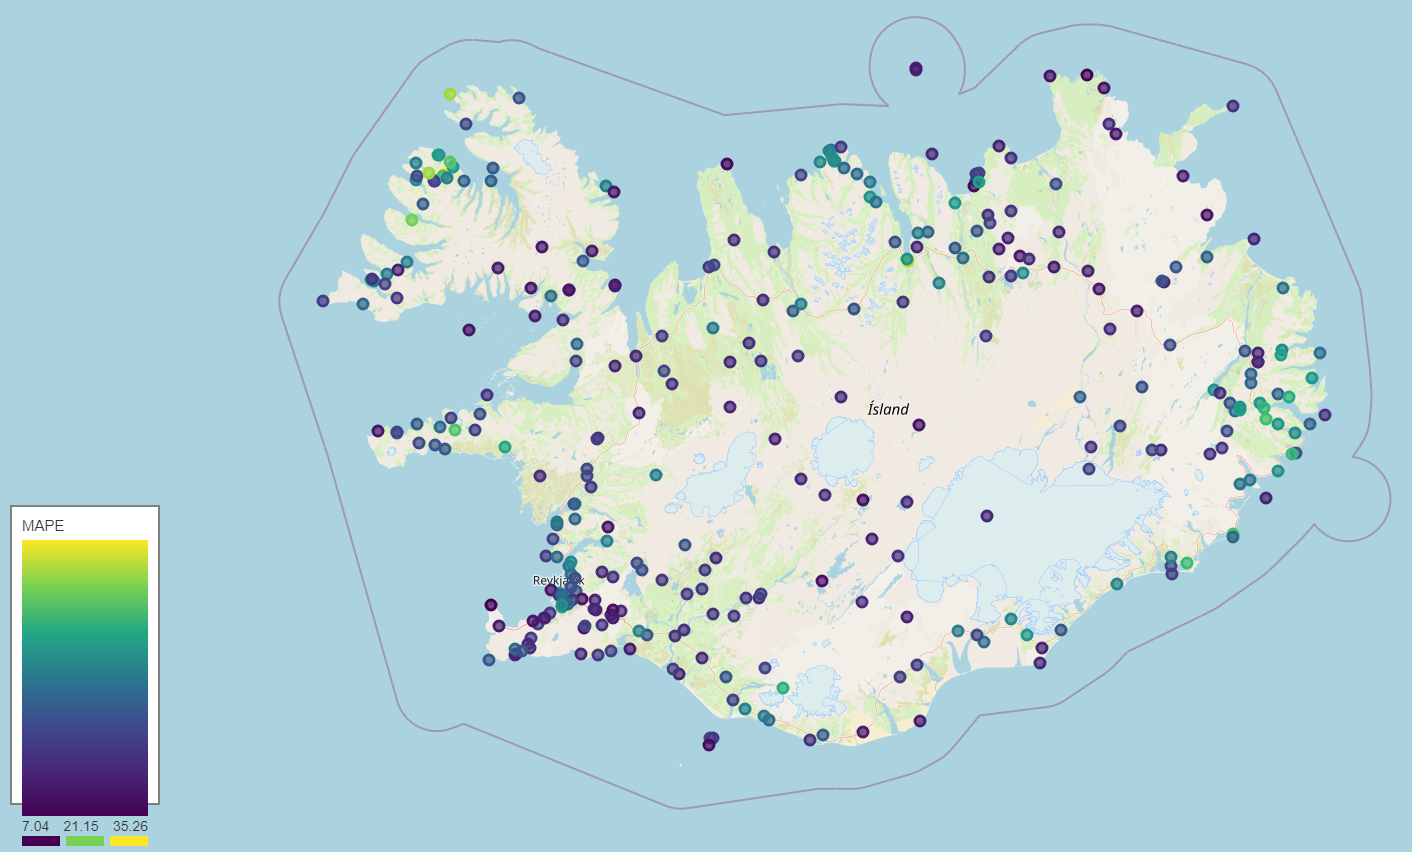
\includegraphics[scale = 0.5]{Figures/errorMap.png}
    \caption[MAPE error distribution of stations shown on a map of Iceland.]{The MAPE error of each station in data shown as color gradient circles. That is each station is represented by one circle, with the error value represented as a color gradient from dark blue to yellow. The lowest error at a single station was around 7\% at Garðskagaviti and the highest around 35\% at Seljalandsdalur. It is important to note that the model is trained using a cutoff of 10 m/s and this cutoff point is determined using the reanalysis wind at 15 meters above ground.}
    \label{fig:errorMap}
\end{figure}

\begin{table}[h]
    \caption[Model result looking at closed wind speed intervals]{The MAPE results for different wind speed limit intervals. Here instead of training for all data above a certain threshold of wind speed, training is done only on data between two wind speeds. The percentage variance in gust factor as a function of wind speed increases with decreasing wind speed. Measured wind speed is used for the cutoff and thus have data leakage. These results should thus be somewhat comparable to the last column in Table (\ref{table:results})}
    \label{table:closed_intervals}
    \centering
    \begin{tabular}{lcc}
        \toprule
        Interval &  \multicolumn{2}{c}{MAPE}\\
        $[m/s]$ & Without Elevation & With Elevation\\
        \midrule
        $[5, 10[$ & 17.1\% & 16.4\%\\
        $[10, 15[$ & 14.5\% & 13.0\%\\
        $[15, 20[$ & 15.0\% & 12.0\%\\
        $[20, 25[$ & 15.6 \% & 13.1\%\\
        $[25, 30[$ & 18.4\% & 19.0\%\\
        \bottomrule
    \end{tabular}
\end{table}

Table (\ref{table:closed_intervals}) shows no improvement over the values in the last column in Table (\ref{table:results}). As previously mentioned, the gust factor decreases with increasing wind speed and thus, training on intervals and lessening this effect might be expected to give better results. This does not seem to be the case. Some interesting sites to look closer at for drivers might include places such as Ingólfsfjall, Kjalarnes and others. These can be seen in Table (\ref{table:more_specific_sites}).

\begin{table}[h]
    \caption[Model result by stations of interest]{The MAPE results of different stations for several stations of interest, both when training for the specific site and when the stations are a part of the general data. For every station the wind speed limit is set at 10 m/s. In training for a single station at a time, some site specific information can be gauged. This does not mean that the a better result can be reached for that site. Factors such as the number of datapoints at given location can significantly impact the result. This table uses the measured wind speed to determine the cut off for data points. This leads to some data leakage and an increased performance compared to using the reanalysis CARRA speed for cut off.}
    \label{table:more_specific_sites}
    \centering
    \begin{tabular}{lcc}
        \toprule
        Station name & \multicolumn{2}{c}{MAPE}\\
         & Baseline & Model\\
        \midrule
        Fáskrúðsfjörður & 28.2\% & 21.8\%\\
        Ingólfsfjall & 30.0\% & 19.6\%\\
        Kjalarnes & 20.7\% & 13.5\% \\
        Sandskeið & 13.0\% & 10.2\%\\
        Seyðisfjörður & 32.1\% & 23.0\%\\
        Þjórsárdalur & 12.2\% & 11.4\%\\
        Þrengsli & 13.6\% & 11.3\%\\
        \bottomrule
    \end{tabular}
\end{table}

\section{Comparison for models with variable parameters}

In Figure (\ref{fig:ShapleySummary}) the contribution of each feature, excluding the elevation points, can be seen for the model in general (a significant subset of data is used). Looking at Figure (\ref{fig:ShapleySummary}), there is an outlier. Exactly calculating the Shapley values is time intensive, in the subset shown there is an outlier that skews the figure and makes it so that viewing the importance distribution excluding the outlier is difficult. For this reason, another shapley summary was created that looked at different, and larger distribution. This can be seen in Figure (\ref{fig:ShapleySummary2}). The Figures (\ref{fig:ShapleySummary}) and (\ref{fig:ShapleySummary2}) show the summary for a model trained only on the features shown and not on landscape elevation of the surrounding area. This is done as the number of points there is too high to display in one figure (70 total points). Looking specifically at Figure (\ref{fig:ShapleySummary2}), the station elevation is most influential and the Richardson number's influence is very low. Most of the feature values bunch up in the middle, while the station elevation is elongated compared to other features. Station elevation seems to have two bunches on either side of 0. Overall, the values seem to be skewed to the right of 0. This would be expected as the predicted values are expected to be in the range of 1.2-2, or at least always above 1 by definition. Finally, for the Shapley values, looking that all the data there are again outliers that skew the data so that spotting general distribution is difficult. This can be seen in Figure (\ref{fig:ShapleySummary3}).

\begin{figure}
    \centering
    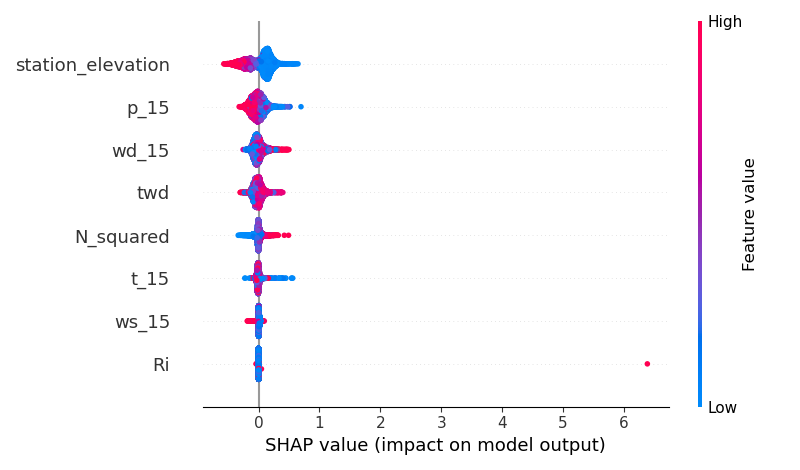
\includegraphics[scale = 0.6]{Figures/shap_plots/summary_plot.png}
    \caption[Summary feature importance of a neural network.]{Feature importance of a neural network with model architecture as described in Table \ref{table:gridSearchHyperparamters} and data as described in Table \ref{table:trainDataExample}. We can see that generally multiple factors influence the prediction, with the station elevation being highly influential. There is seemingly one outlier for the Richardson number, which usually has very little influence. Elevation data is excluded when working with Shapley values, as the contribution of each elevation point is very low and there are very many of them. To see their influence on the model output see Table \ref{table:results}.}
    \label{fig:ShapleySummary}
\end{figure}

\begin{figure}
    \centering
    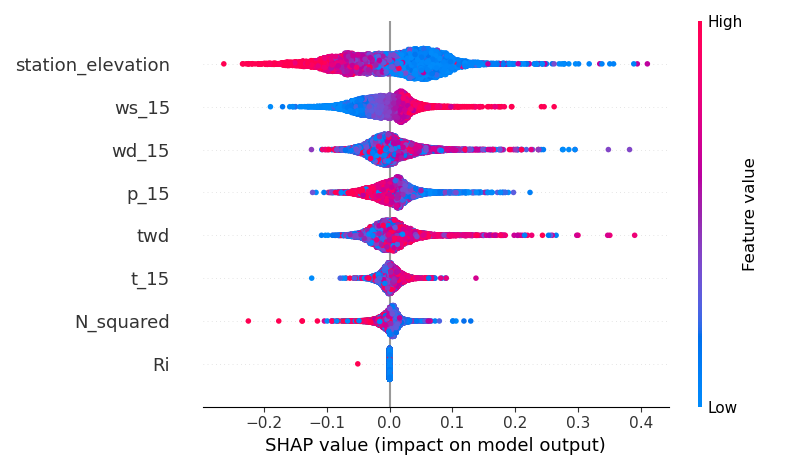
\includegraphics[scale = 0.6]{Figures/shap_plots/summary_plot_190924_.png}
    \caption[Summary feature importance of a neural network using a larger distribution of data.]{Feature importance of a neural network with model architecture as described in Table \ref{table:gridSearchHyperparamters} and data as described in Table \ref{table:trainDataExample}. Generally multiple factors influence the prediction, with the station elevation being highly influential. Elevation data is excluded when working with Shapley values, as the contribution of each elevation. In contrast to Figure (\ref{fig:ShapleySummary}), the distribution doesn't have as extreme outliers. This means that more details can be seen in the figure. The X-axis shows the influence of feature values on the model. The color gradient shows the value of each feature. As an example, there is a very red value for station elevation (top line, all the way to the left). This means that in this instance, the station elevation contributed around -0.25 to the final output and that the station had an elevation significantly above average.}
    \label{fig:ShapleySummary2}
\end{figure}

Further Shapley figures can be seen in Appendix~\ref{appendix:A}. In each of these plots, even without the feature labels, the station elevation is easily noticed as the value is constant for a station. This is not noteworthy. What is noteworthy is the range of impact from this single value. For simpler models, this would not happen. It is important to note that SHAP assumes feature independence\cite{Salih_2024}. This might explain why the impact of the Richardson number is so low. Both the squared Brunt–Väisälä frequency and the Richardson number are derived features from reanalysis data. They carry with them some extra information over the other features in the dataset. This is because both are variables over elevation ranges. That is, as seen in Equations (\ref{eqn:Ri}, \ref{eqn:N}), both are dependent on values at lower and upper elevations and try to describe the stability of that range. Shapley tries to assign contribution values for each feature for each observation. SHAP assumes that the features are independent, but this is not the case. It is clearly not the case for the derived variables, but how the contribution should be distributed between the features is not clear. Seemingly the SHAP python package is giving all the impact to the Brunt–Väisälä squared frequency and none to Richardson number. If the Brunt–Väisälä would be excluded from the data, the impact of the Richardson number would likely increase. Another point to note is that the features are ordered by their impact. This means that the station elevation is the most impactful for each plot, but the ordering of other variables changes. Looking at Figure (\ref{fig:ShapleySummary3}), which shows the Shapley summary plot for all data, the wind speed is the second most important feature. This is reversed in Figure (\ref{fig:ShapleySummaryAkrafjall}). This is not unexpected as Akrafjall station was specifically selected as the MAE for reanalysis wind speed was very high as can be seen in Table (\ref{fig:ShapleySummaryAkrafjall}), where you will also find the stations whose summary plot is shown in Figures (\ref{fig:ShapleySummaryAlmannaskarð}, \ref{fig:ShapleySummaryAsgarðsfjall}) and these also fall into the category of very high MAE for wind speed. What is interesting is that the reanalysis wind speed is also of low impact at stations like Háahlíð and Keflavíkurflugvöllur, as shown in Figures (\ref{fig:ShapleySummaryHaahlid}, \ref{fig:ShapleySummaryKeflavikurflugvollur}). These stations had the lowest of MAE for difference between measured wind speed and reanalysis wind speed. As the summary plot over all stations (Figure (\ref{fig:ShapleySummary3})) shows that reanalysis wind speed is impactful, might lead to the conclusion that the reanalysis wind speed is not a good predictor at these locations or something else is skewing the data. A simpler way to look at feature importance is to create models that are trained on and use to predict different sets of parameters. The results of such a comparison can be seen in Table \ref{table:setsOfParams}.

